\section{Deployment} \thispagestyle{nomarkstyle}
Im Verlauf der Entwicklung stellte sich intern das Bedürfnis nach einer durchgehend lauffähigen Online-Demo des Webshops heraus. Dabei sollten alle Änderungen am Projekt automatisch compiliert und in das Demo-System eingespielt werden. Um dies umsetzen zu können wurde eine Deployment-Strategie definiert, die in diesem Abschnitt näher erläutert wird.

\subsection{Versionsverwaltung mit Git}
Für die Versionsverwaltung des Projekts wird Git verwendet, eines der beliebtesten Versionsverwaltungssysteme in der Softwareentwicklung. Als zentrale Ablage des Quellcodes wurde ein Repository in der GitHub-Plattform erstellt, sodass die Teammitglieder bequem ihre Änderungen an das Repository senden und auch die neuesten Änderungen aktualisieren können\cite{Coutermarsh2014}. Neben den allgemeinen Vorteilen von Git und GitHub ist deren Einsatz auch eine Voraussetzung für die nächsten Schritte.

\subsection{Travis Continuous Integration}
Die Travis CI (Continuous Integration) Software ermöglicht es automatisch bei einem Commit auf das GitHub Repository die Anwendung zu bauen (inklusive Test-Suites falls welche konfiguriert sind). Zudem kann Travis auch so eingestellt werden, dass nach einem erfolgreichen Build der Code direkt in die gewünschte Umgebung deployed wird\cite{Coutermarsh2014}.

Die Einrichtung von Travis ist in wenigen Schritten erledigt:

\begin{enumerate}
	\item Je nachdem ob es sich um ein Open Source oder ein privates Repository handelt ist eine Anmeldung mit dem GitHub-Konto über jeweils \textit{travis-ci.org} oder \textit{travis-ci.com} nötig. In diesem Fall handelt es sich um ein Open Source Projekt.
	\item In der Profilübersicht sind alle Repositories des angemeldeten Benutzerkontos aufgelistet. Anhand eines Buttons kann Travis für das entsprechende Repository aktiviert werden. Dadurch wird ein sogenanntes \enquote{Webhook} gesetzt, welches zukünftige Commits erkennt und automatisch ein Build ausführt.
	\item Im Hauptverzeichnis des Repositories muss eine Datei mit dem Namen \texttt{.travis.yml} erstellt werden. Diese Datei teilt Travis mehrere Informationen die für den Build benötigt werden, wie die verwendete Programmiersprache, weitere Befehle die ausgeführt werden sollen und die Deployment-Konfigurationen.
\end{enumerate}

Der Inhalt der \textit{.travis.yml}-Datei für dieses Projekt ist in Anhang \ref{appendix:travis_yaml} zu finden. Ein wichtiger Schritt des automatisierten Builds ist die Ausführung des \texttt{ng build} Befehls von Angular, der bereits in \cref{angular_setup} erwähnt wurde. Darauf folgt ein automatischer Commit der generierten Ressourcen für die Angular-Anwendung und zuletzt das Deployment der gesamten Applikation auf die Server-Instanz (in diesem Fall von Heroku).

\subsection{Heroku}
Ursprünglich war es gedacht, einen eigenen privaten Webserver für das Deployment des Webshops einzurichten. Es wurde jedoch schnell klar, dass der Aufwand im Verhältnis zur sehr geringen erreichten Performanz viel zu hoch wurde. Dadurch fiel die Entscheidung dafür, eine Cloud-Lösung zu verwenden. Das geeignetste Service-Modell in diesem Anwendungsfall war \textit{Platform as a Service} (PaaS). Diese Dienstleistung stellt alle notwendige Infrastrukturkomponenten wie Server, Speicher und Netzwerkelemente zur Verfügung, sowie zusätzlich Middleware, Entwicklungstools, BI-Dienste (Business Intelligence), Datenbank-Verwaltungssysteme und mehr\cite{Azure2017}. Zur Veranschaulichung sind auf \cref{fig:cloud} die Unterschiede zwischen den drei Servicemodellen des Cloud Computings dargestellt: Software as a Service (SaaS), Platform as a Service (PaaS) und Infrastructure as a Service (IaaS).

\begin{figure}[th!]
	\centering
	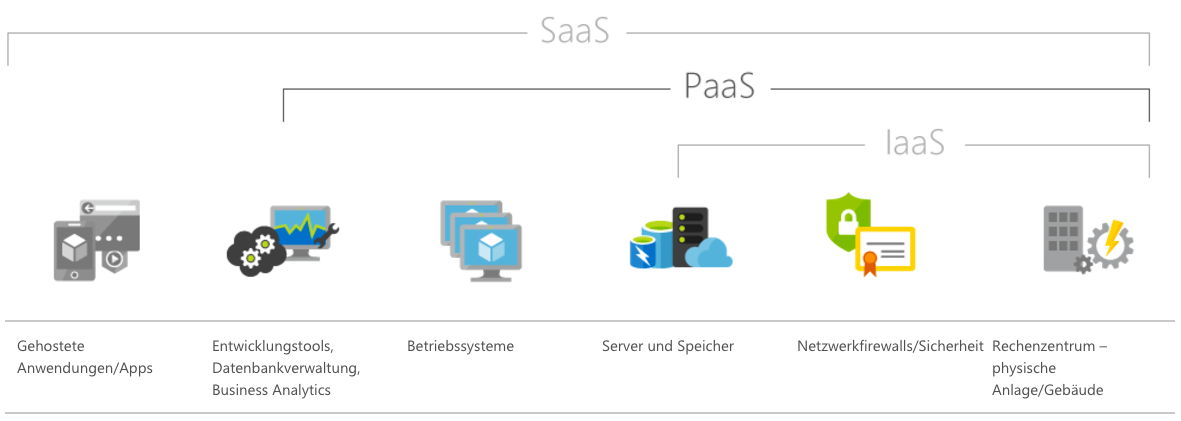
\includegraphics[width=\linewidth]{bilder/kap8/cloud}
	\caption[Bestandteile der Cloud-Servicemodelle]{Bestandteile der Cloud-Servicemodelle\cite{Azure2017}}
	\label{fig:cloud}
\end{figure}

Im PaaS-Umfeld ist Heroku einer der beliebtesten Anbietern. Das Erstellen eines virtuellen Webservers (in Heroku \textit{Dyno} genannt) ist sehr einfach und auch das automatische Deployment von Travis nach Heroku funktioniert reibungslos. Zudem werden inzwischen einige Programmiersprachen und auch Frameworks wie Spring unterstützt\cite{Coutermarsh2014}.

Wie bei vielen anderen Cloud-Anbietern werden bei Heroku unterschiedliche Tarife vermarktet, die entsprechend mehr oder weniger Dienstleistungen umfassen. Für dieses Projekt war der kostenlose Tarif völlig ausreichend. Dieser enthält ein Dyno mit 512MB RAM, was für den Anwendungsfall genügt. 

\subsection{AWS Datenbank Instanz}

Auch hier war es einst geplant einen privaten Datenbank-Server einzurichten und verfügbar zu machen, jedoch waren letztendlich die Performanz und die Stabilität des Servers annehmbar. Eine interessante Alternative dazu bot Amazon Web Services (\acs{AWS}), bzw. konkret deren Amazon Relational Database Service (Amazon RDS). Das Produkt ermöglicht es, relationale Datenbanken einfach zu erstellen, zu verwalten und zu skalieren\cite{Gaut2016}. Über die Weboberfläche von Amazon RDS konnte für das Projekt in wenigen Schritten eine kostenfreie MySQL Datenbank-Instanz mit 5GB Speicherplatz und 1GB RAM angelegt werden.
